% ============================================================
%  يُترجَم بـ XeLaTeX  (في Overleaf: Menu → Compiler → XeLaTeX)
%  الخط: Amiri (متوفر في Overleaf، أو حمّله من github.com/aliftype/amiri)
% ============================================================
\documentclass[12pt,a4paper]{article}
\usepackage[a4paper,margin=1.7cm,top=2.3cm,bottom=2.9cm,headheight=15pt,footskip=1.5cm]{geometry}
\usepackage{amsmath,amssymb}
\usepackage{icomma}
\usepackage[english,bidi=default,layout=lists]{babel}
\babelprovide[import,main]{arabic}
\babelfont{rm}[Scale=1.08]{Amiri}
\babelfont{sf}[Scale=1.08]{Amiri}
\usepackage[most]{tcolorbox}
\usepackage{tikz}
\usetikzlibrary{arrows.meta,calc,shadings}
\usepackage{array}
\usepackage{colortbl}
\usepackage{fancyhdr}
\usepackage{titlesec}
\usepackage{enumitem}
\usepackage{collcell}
\usepackage{needspace}
\usepackage{etoolbox}
\newcolumntype{C}{>{\collectcell\ar}c<{\endcollectcell}}
\pretocmd{\section}{\Needspace{15\baselineskip}}{}{}
\pretocmd{\subsection}{\Needspace{11\baselineskip}}{}{}

\definecolor{cDef}{HTML}{1F4E9C}
\definecolor{cThm}{HTML}{B3261E}
\definecolor{cRem}{HTML}{2E7D32}
\definecolor{cEx}{HTML}{C76B00}
\definecolor{cMeth}{HTML}{6A1B9A}
\definecolor{cSol}{HTML}{00695C}
\definecolor{cSec}{HTML}{1F3A68}

\titleformat{\section}{\Large\bfseries\color{cSec}}{\thesection.}{0.6em}{}[{\color{cSec!60}\titlerule[1pt]}]
\titleformat{\subsection}{\large\bfseries\color{cThm!85!black}}{\thesubsection.}{0.5em}{}
\titlespacing*{\section}{0pt}{14pt}{8pt}
\titlespacing*{\subsection}{0pt}{10pt}{5pt}
\setlength{\parindent}{0pt}
\setlength{\parskip}{4pt}
\setlist{itemsep=2pt,topsep=3pt}

\newtcolorbox{arbox}[3][]{enhanced,
  colback=#2!5,colframe=#2!80!black,arc=2mm,boxrule=0.8pt,
  left=6pt,right=6pt,top=8pt,bottom=5pt,
  fonttitle=\bfseries,coltitle=white,
  title={\foreignlanguage{arabic}{#3}},
  attach boxed title to top right={xshift=-5mm,yshift=-3mm},
  boxed title style={colback=#2!80!black,arc=1.5mm,boxrule=0pt},
  before upper={\selectlanguage{arabic}},
  before skip=8pt,after skip=8pt,breakable,#1}
\newenvironment{BOX}[2]{\begin{otherlanguage}{english}\begin{arbox}{#1}{#2}}{\end{arbox}\end{otherlanguage}}
\newenvironment{tarif}[1][تعريف]{\begin{BOX}{cDef}{#1}}{\end{BOX}}
\newenvironment{khassia}[1][خاصية]{\begin{BOX}{cThm}{#1}}{\end{BOX}}
\newenvironment{molahada}[1][ملاحظة]{\begin{BOX}{cRem}{#1}}{\end{BOX}}
\newenvironment{mithal}[1][مثال]{\begin{BOX}{cEx}{#1}}{\end{BOX}}
\newenvironment{tariqa}[1][طريقة]{\begin{BOX}{cMeth}{#1}}{\end{BOX}}

\newcounter{exo}
\newenvironment{tamrin}[1]{\stepcounter{exo}\begin{BOX}{cSec}{التمرين \theexo: #1}}{\end{BOX}}
\newenvironment{hal}{\Needspace{12\baselineskip}\begin{otherlanguage}{english}\begin{arbox}[breakable]{cSol}{حل التمرين \theexo}}{\end{arbox}\end{otherlanguage}}

\newenvironment{LTR}{\begin{otherlanguage}{english}}{\end{otherlanguage}}
\newcommand{\ar}[1]{\foreignlanguage{arabic}{#1}}

\renewcommand{\dots}{\mathinner{\ldotp\ldotp\ldotp}}
\renewcommand{\ldots}{\mathinner{\ldotp\ldotp\ldotp}}
\renewcommand{\cdots}{\mathinner{\cdotp\cdotp\cdotp}}
\newcommand{\N}{\mathbb{N}}
\newcommand{\Z}{\mathbb{Z}}
\newcommand{\D}{\mathbb{D}}
\newcommand{\Q}{\mathbb{Q}}
\newcommand{\R}{\mathbb{R}}
\newcommand{\pgcd}{\operatorname{PGCD}}
\newcommand{\ppcm}{\operatorname{PPCM}}

% \NLseg{a}{b}{[}{]} ; \NLright{a}{[} ; \NLleft{b}{]}  (interval on a number line)
\newcommand{\NLseg}[4]{\begin{LTR}\begin{tikzpicture}[baseline=-0.6ex]
 \draw[-{Stealth[length=2mm]},gray!70](0,0)--(3.4,0);
 \draw[line width=2pt,cThm!80!black](0.7,0)--(2.7,0);
 \node[cThm!80!black,font=\LARGE] at (0.7,0){$#3$};
 \node[cThm!80!black,font=\LARGE] at (2.7,0){$#4$};
 \node[below=3pt,font=\footnotesize] at (0.7,0){$#1$};
 \node[below=3pt,font=\footnotesize] at (2.7,0){$#2$};
\end{tikzpicture}\end{LTR}}
\newcommand{\NLright}[2]{\begin{LTR}\begin{tikzpicture}[baseline=-0.6ex]
 \draw[-{Stealth[length=2mm]},gray!70](0,0)--(3.4,0);
 \draw[line width=2pt,cThm!80!black](1.3,0)--(3.3,0);
 \node[cThm!80!black,font=\LARGE] at (1.3,0){$#2$};
 \node[below=3pt,font=\footnotesize] at (1.3,0){$#1$};
\end{tikzpicture}\end{LTR}}
\newcommand{\NLleft}[2]{\begin{LTR}\begin{tikzpicture}[baseline=-0.6ex]
 \draw[-{Stealth[length=2mm]},gray!70](0,0)--(3.4,0);
 \draw[line width=2pt,cThm!80!black](0.05,0)--(2.1,0);
 \node[cThm!80!black,font=\LARGE] at (2.1,0){$#2$};
 \node[below=3pt,font=\footnotesize] at (2.1,0){$#1$};
\end{tikzpicture}\end{LTR}}

% ---------- social-media icons (pure TikZ) ----------
\definecolor{cFB}{HTML}{1877F2}
\definecolor{cTG}{HTML}{229ED9}
\definecolor{cIG1}{HTML}{FEDA75}
\definecolor{cIG2}{HTML}{D62976}
\definecolor{cIG3}{HTML}{4F5BD5}
\newcommand{\fbicon}{\begin{LTR}\begin{tikzpicture}[baseline=-0.75ex,x=1em,y=1em]
 \fill[cFB] (0,0) circle (0.55);
 \node[white,inner sep=0,font=\usefont{TU}{lmss}{bx}{n}\small] at (0.04,-0.02) {f};
\end{tikzpicture}\end{LTR}}
\newcommand{\igicon}{\begin{LTR}
\begin{tikzpicture}[baseline=-0.75ex,x=1em,y=1em]
 \shade[lower left=cIG1,lower right=cIG2,upper left=cIG2,upper right=cIG3,rounded corners=0.28em] (-0.55,-0.55) rectangle (0.55,0.55);
 \draw[white,line width=0.09em,rounded corners=0.18em] (-0.36,-0.36) rectangle (0.36,0.36);
 \draw[white,line width=0.09em] (0,0) circle (0.17);
 \fill[white] (0.22,0.22) circle (0.05);
\end{tikzpicture}\end{LTR}}
\newcommand{\tgicon}{\begin{LTR}
\begin{tikzpicture}[baseline=-0.75ex,x=1em,y=1em]
 \fill[cTG] (0,0) circle (0.55);
 \fill[white] (-0.33,0.0) -- (0.32,0.27) -- (0.2,-0.3) -- (0.0,-0.15) -- (-0.08,-0.28) -- (-0.08,-0.08) -- cycle;
 \fill[cTG!70!black] (-0.08,-0.08) -- (0.25,0.2) -- (0.0,-0.15) -- (-0.08,-0.28) -- cycle;
\end{tikzpicture}\end{LTR}}
% page number: black box, white two-digit number, at the right of the social row
\newcommand{\PageBox}{\begin{LTR}\tikz[baseline=(p.base)]\node[fill=black,text=white,inner sep=2.5pt,minimum width=1.6em,minimum height=1.3em,font=\usefont{TU}{lmss}{bx}{n}\small](p){\ifnum\value{page}<10 0\fi\arabic{page}};\end{LTR}}
% visual left-to-right order: Telegram | Instagram | Facebook | page box
\newcommand{\SocialRow}{\begin{otherlanguage}{english}%
 \ar{\textbf{الأستاذ سوايسية هشام للرياضيات}}\ \tgicon\hfill
 \textbf{prof\_hicham\_math}\ \igicon\hfill
 \ar{\textbf{الأستاذ سوايسية هشام للرياضيات}}\ \fbicon\hspace{2.2em}\PageBox\end{otherlanguage}}

\pagestyle{fancy}
\fancyhf{}
\renewcommand{\headrulewidth}{0.6pt}
\renewcommand{\footrulewidth}{0.4pt}
% \SetHeader{right head: document title}{left head: level -- stream}
\newcommand{\SetHeader}[2]{%
 \fancyhead[C]{\parbox{\textwidth}{\ar{#1\hfill #2}}}%
 \fancyfoot[C]{\PageBox}}
\usepackage{tkz-tab}
\usepackage{multicol}
% variation / sign table (LTR)
\newenvironment{TAB}{\par\begin{center}\begin{LTR}\begin{tikzpicture}[scale=0.95,every node/.style={font=\small}]}{\end{tikzpicture}\end{LTR}\end{center}}
% grid + axes, clipped: \begin{GR}{xmin}{xmax}{ymin}{ymax}{unit cm}
\newenvironment{GR}[5]{\par\begin{center}\begin{LTR}\begin{tikzpicture}[x=#5cm,y=#5cm,font=\footnotesize]
 \draw[gray!25,very thin] (#1,#3) grid (#2,#4);
 \draw[-{Stealth[length=2mm]}] (#1,0)--(#2+0.3,0) node[below left]{$x$};
 \draw[-{Stealth[length=2mm]}] (0,#3)--(0,#4+0.3) node[below left]{$y$};
 \node[below left] at (0,0){$O$};
 \begin{scope}\clip (#1,#3) rectangle (#2,#4);}
{\end{scope}\end{tikzpicture}\end{LTR}\end{center}}
\newcommand{\Ticks}[2]{\foreach \t in {#1} \node[below,font=\scriptsize] at (\t,0){$\t$}; \foreach \t in {#2} \node[left,font=\scriptsize] at (0,\t){$\t$};}
\newcommand{\bx}[1]{\ensuremath{\setlength{\fboxsep}{2pt}\fcolorbox{cEx!85!black}{yellow!35}{$\displaystyle #1$}}}
\newcommand{\TwoCol}[4]{\par\begin{LTR}\noindent\begin{minipage}[t]{#1\textwidth}\selectlanguage{arabic}#2\end{minipage}\hfill\begin{minipage}[t]{#3\textwidth}\selectlanguage{arabic}#4\end{minipage}\end{LTR}\par}
\newcommand{\RL}[4]{\TwoCol{#3}{#4}{#1}{#2}}  % \RL{w1}{right content}{w2}{left content}
\newcommand{\ok}{$\textcolor{cRem}{\checkmark}$}
\newcommand{\limn}{\displaystyle\lim_{n\to+\infty}}
% sub-questions, each on its own line
\newenvironment{sq}{\begin{itemize}[leftmargin=2.4em,itemsep=3pt]}{\end{itemize}}
\newcommand{\qa}{\item[(أ)]}\newcommand{\qb}{\item[(ب)]}\newcommand{\qc}{\item[(جـ)]}\newcommand{\qd}{\item[(د)]}\newcommand{\qe}{\item[(هـ)]}
\newcommand{\pa}{\par\smallskip\textbf{(أ)} }\newcommand{\pb}{\par\smallskip\textbf{(ب)} }\newcommand{\pc}{\par\smallskip\textbf{(جـ)} }\newcommand{\pd}{\par\smallskip\textbf{(د)} }\newcommand{\pe}{\par\smallskip\textbf{(هـ)} }
\newcommand{\QQ}[1]{\par\smallskip\textbf{#1.} }
\newenvironment{tmr}{\stepcounter{exo}\begin{BOX}{cSec}{تمرين محلول \theexo}}{\end{BOX}}
\newcommand{\ABC}[3]{\\[2pt]\begin{tabular}{p{0.28\textwidth}p{0.28\textwidth}p{0.28\textwidth}}(جـ) \ #3 & (ب) \ #2 & (أ) \ #1\end{tabular}}

\newcommand{\nt}[1]{\hfill$\textcolor{cThm}{\mathbf{(#1)}}$}
\SetHeader{\small\bfseries\color{cSec}فرض المراقبة الذاتية رقم 01}{\small\color{cSec}السنة الثانية ثانوي -- تقني رياضي ورياضيات}
\begin{document}
\begin{center}
{\large\bfseries الجمهورية الجزائرية الديمقراطية الشعبية}\\[2pt]
{\bfseries وزارة التربية الوطنية}\\[2pt]
{\bfseries الديوان الوطني للتعليم والتكوين عن بعد}\\[2pt]
{\bfseries المركز الولائي سوق أهراس}
\end{center}
\noindent\textbf{السنة الدراسية: 2026/2027}\hfill\textbf{المستوى: سنة ثانية ثانوي شعبة تقني رياضي ورياضيات}
\par\smallskip
\begin{LTR}
\begin{tcolorbox}[enhanced,colback=cSec,colframe=cSec,arc=2mm,halign=center,boxrule=0pt,top=6pt,bottom=6pt,before upper={\selectlanguage{arabic}}]
{\color{white}\Large\bfseries فرض المراقبة الذاتية رقم 01 -- الموضوع الثاني}
\end{tcolorbox}
\end{LTR}

\begin{tamrin}{الاشتقاقية: دستور الدالة (07 نقاط)}
$f$ الدالة المعرّفة على $\R-\{-1\}$ بـ: $f(x)=\dfrac{x^2+x+4}{x+1}$ ، و $(C_f)$ تمثيلها البياني في معلم متعامد ومتجانس.
\QQ{1} باستعمال تعريف العدد المشتق ، بيّن أن $f$ قابلة للاشتقاق عند $0$ وأن: $f^{\prime}(0)=-3$.
\QQ{2} اكتب معادلة للمماس $(T)$ للمنحنى $(C_f)$ عند النقطة ذات الفاصلة $0$ ، ثم استنتج قيمة تقريبية للعدد $f(0{,}01)$.
\QQ{3} بيّن أنه من أجل كل $x\neq-1$: $f^{\prime}(x)=\dfrac{(x-1)(x+3)}{(x+1)^2}$.
\QQ{4} ادرس اتجاه تغيّر الدالة $f$ ، ثم شكّل جدول تغيّراتها (دون حساب النهايات) ، وعيّن قيمها الحدية المحلية.
\QQ{5} تحقّق أنه من أجل كل $x\neq-1$: $f(x)=x+\dfrac4{x+1}$ ، ثم عيّن فواصل النقط من $(C_f)$ التي يكون فيها المماس موازياً للمستقيم $(T)$.
\QQ{6} \textbf{(سؤال تميّز)} عيّن فاصلة النقطة من $(C_f)$ التي يشمل المماس عندها مبدأ المعلم $O$ ، ثم اكتب معادلة هذا المماس.
\end{tamrin}

\begin{tamrin}{الاشتقاقية: قراءة بيانية (05 نقاط)}
$(C_g)$ التمثيل البياني لدالة $g$ معرّفة وقابلة للاشتقاق على $\R$. المستقيم $(T)$ مماس لـ $(C_g)$ عند النقطة $A(0;1)$ ويشمل النقطة $B(1;-2)$ ، والمماسان عند النقطتين ذات الفاصلتين $-1$ و $1$ يوازيان محور الفواصل.
\begin{center}\begin{LTR}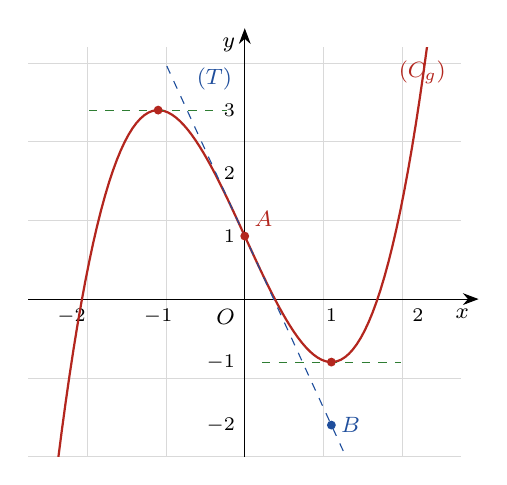
\begin{tikzpicture}[x=1.1cm,y=0.8cm,font=\footnotesize]
\draw[gray!30,very thin] (-2.5,-2.5) grid (2.5,4);
\draw[-{Stealth[length=2mm]}] (-2.5,0)--(2.7,0) node[below left]{$x$};
\draw[-{Stealth[length=2mm]}] (0,-2.5)--(0,4.3) node[below left]{$y$};
\foreach \t in {-2,-1,1,2} \node[below,font=\scriptsize] at (\t,0){$\t$};
\foreach \t in {-2,-1,1,2,3} \node[left,font=\scriptsize] at (0,\t){$\t$};
\node[below left] at (0,0){$O$};
\begin{scope}\clip (-2.5,-2.5) rectangle (2.5,4);
\draw[cThm,thick,domain=-2.25:2.25,samples=100] plot (\x,{\x*\x*\x-3*\x+1});
\draw[cDef,dashed] (-0.9,3.7)--(1.4,-3.2);
\draw[cRem,dashed] (-1.8,3)--(-0.2,3); \draw[cRem,dashed] (0.2,-1)--(1.8,-1);
\end{scope}
\fill[cThm] (-1,3) circle (1.6pt) (1,-1) circle (1.6pt) (0,1) circle (1.6pt); \fill[cDef] (1,-2) circle (1.6pt) node[right]{$B$}; \node[cThm,above right] at (0,1){$A$};
\node[cThm] at (2.05,3.6){$(C_g)$}; \node[cDef] at (-0.35,3.5){$(T)$};
\end{tikzpicture}\end{LTR}\end{center}
\QQ{1} بقراءة بيانية عيّن: $g(-1)$ ، $g(0)$ ، $g(1)$ ، $g^{\prime}(-1)$ ، $g^{\prime}(1)$.
\QQ{2} احسب $g^{\prime}(0)$ ، ثم اكتب معادلة للمماس $(T)$.
\QQ{3} شكّل جدول تغيّرات الدالة $g$ على المجال $[-2;2]$ ، ثم استنتج إشارة $g^{\prime}(x)$.
\QQ{4} نقبل أن $g(x)=x^3+ax+b$. باستعمال النتائج السابقة عيّن العددين الحقيقيين $a$ و $b$.
\QQ{5} حدّد بيانياً عدد حلول المعادلة $g(x)=0$ في المجال $[-2;2]$.
\QQ{6} \textbf{(سؤال تميّز)} ناقش بيانياً ، حسب قيم الوسيط الحقيقي $m$ ، عدد حلول المعادلة $g(x)=m$ في المجال $[-2;2]$.
\end{tamrin}

\begin{tamrin}{الاحتمالات (08 نقاط)}
نرمي مرتين متتاليتين حجر نرد رباعي الوجوه منتظماً ، وجوهه مرقمة من $1$ إلى $4$ ، ونسجّل الرقم الظاهر على الوجه المخفي في كل رمية.
\QQ{1} مثّل مجموعة الإمكانيات بجدول ذي مدخلين ، ثم عيّن عددها.
\QQ{2} احسب احتمال كل حادثة من الحوادث التالية:
\begin{sq}
\qa $A$: «الرقمان متساويان».
\qb $B$: «مجموع الرقمين يساوي $5$».
\qc $C$: «الرقم $4$ يظهر مرة واحدة على الأقل».
\qd $A\cup C$.
\end{sq}
\QQ{3} ليكن $X$ المتغير العشوائي الذي يرفق بكل نتيجة أكبر الرقمين المسجلين (وإذا تساويا نأخذ الرقم نفسه).
\begin{sq}
\qa عيّن القيم الممكنة للمتغير العشوائي $X$ ، ثم عرّف قانون احتماله.
\qb احسب الأمل الرياضياتي $E(X)$ ، والتباين $V(X)$ ، والانحراف المعياري $\sigma(X)$.
\end{sq}
\QQ{4} يدفع لاعب $m$ دينار ليرمي الحجر مرتين ، ويتحصل على $8X$ دينار. عيّن قيمة $m$ التي تجعل اللعبة عادلة.
\QQ{5} \textbf{(سؤال تميّز)} نغيّر قاعدة اللعبة: يربح اللاعب $a$ دينار إذا ظهر الرقم $4$ مرة واحدة على الأقل ، ويخسر $7$ دنانير في الحالة المعاكسة. عيّن $a$ لتكون اللعبة عادلة.
\end{tamrin}
\begin{center}\textbf{\color{cSec}بالتوفيق}\end{center}

\newpage
\begin{LTR}
\begin{tcolorbox}[enhanced,colback=cSol,colframe=cSol,arc=2mm,halign=center,boxrule=0pt,top=6pt,bottom=6pt,before upper={\selectlanguage{arabic}}]
{\color{white}\Large\bfseries الحل النموذجي وسلم التنقيط}
\end{tcolorbox}
\end{LTR}
\Needspace{12\baselineskip}\begin{BOX}{cSol}{حل التمرين 1}
\QQ{1} $f(0)=4$. من أجل $h\neq0$ و $h\neq-1$:
\par $\dfrac{f(h)-f(0)}h=\dfrac1h\left(\dfrac{h^2+h+4}{h+1}-4\right)=\dfrac1h\times\dfrac{h^2-3h}{h+1}=\dfrac{h-3}{h+1}$.
\par $\lim\limits_{h\to0}\dfrac{h-3}{h+1}=-3$ (عدد حقيقي) ، إذن $f$ قابلة للاشتقاق عند $0$ و \bx{f^{\prime}(0)=-3} \hfill$\textcolor{cThm}{\mathbf{(1)}}$
\QQ{2} $(T):y=f^{\prime}(0)(x-0)+f(0)$ ، أي \bx{(T):y=-3x+4} \hfill$\textcolor{cThm}{\mathbf{(0,5)}}$
\par التقريب التآلفي: $f(0{,}01)\approx-3(0{,}01)+4=\bx{3{,}97}$ \hfill$\textcolor{cThm}{\mathbf{(0,5)}}$
\QQ{3} $f=\dfrac uv$ مع $u(x)=x^2+x+4$ ، $u^{\prime}(x)=2x+1$ ، $v(x)=x+1$ ، $v^{\prime}(x)=1$:
\par $f^{\prime}(x)=\dfrac{(2x+1)(x+1)-\left(x^2+x+4\right)}{(x+1)^2}=\dfrac{x^2+2x-3}{(x+1)^2}=\bx{\dfrac{(x-1)(x+3)}{(x+1)^2}}$ \hfill$\textcolor{cThm}{\mathbf{(1)}}$
\QQ{4} $(x+1)^2>0$ ، فإشارة $f^{\prime}(x)$ من إشارة $(x-1)(x+3)$: $f(-3)=\dfrac{9-3+4}{-2}=-5$ ، $f(1)=\dfrac{6}{2}=3$.
\begin{TAB}
\tkzTabInit[lgt=1.6,espcl=1.9]{$x$/0.8,$f^{\prime}(x)$/0.8,$f(x)$/1.6}{$-\infty$,$-3$,$-1$,$1$,$+\infty$}
\tkzTabLine{,+,z,-,d,-,z,+,}
\tkzTabVar{-/ ,+/$-5$,-D+/ / ,-/$3$,+/ }
\end{TAB}
$f$ متزايدة تماماً على $]-\infty;-3]$ و $[1;+\infty[$ ، ومتناقصة تماماً على $[-3;-1[$ و $]-1;1]$.
\par قيمة حدية عظمى محلية \bx{f(-3)=-5} ، وقيمة حدية صغرى محلية \bx{f(1)=3} \hfill$\textcolor{cThm}{\mathbf{(1,5)}}$
\QQ{5} $x+\dfrac4{x+1}=\dfrac{x(x+1)+4}{x+1}=\dfrac{x^2+x+4}{x+1}=f(x)$.
\par المماس يوازي $(T)$ معناه $f^{\prime}(x)=-3$: $\dfrac{x^2+2x-3}{(x+1)^2}=-3$ ، أي $x^2+2x-3=-3x^2-6x-3$ ، أي $4x^2+8x=0$ ، أي $4x(x+2)=0$.
\par الفاصلتان: \bx{x=0} (النقطة $A$ نفسها) و \bx{x=-2} \hfill$\textcolor{cThm}{\mathbf{(1)}}$
\QQ{6} معادلة المماس عند النقطة ذات الفاصلة $a$ ($a\neq-1$): $y=f^{\prime}(a)(x-a)+f(a)$. يشمل $O$ معناه $0=-af^{\prime}(a)+f(a)$ ، أي $af^{\prime}(a)=f(a)$:
\par $a\times\dfrac{a^2+2a-3}{(a+1)^2}=\dfrac{a^2+a+4}{a+1}$ ، أي $a\left(a^2+2a-3\right)=\left(a^2+a+4\right)(a+1)$ ، أي $a^3+2a^2-3a=a^3+2a^2+5a+4$ ، ومنه $-8a=4$: \bx{a=-\tfrac12}
\par $f\left(-\tfrac12\right)=\dfrac{\frac14-\frac12+4}{\frac12}=\dfrac{15}2$ ، $f^{\prime}\left(-\tfrac12\right)=\dfrac{\frac14-1-3}{\frac14}=-15$ ، والمماس: \bx{y=-15x} \hfill$\textcolor{cThm}{\mathbf{(1,5)}}$
\end{BOX}

\Needspace{12\baselineskip}\begin{BOX}{cSol}{حل التمرين 2}
\QQ{1} \bx{g(-1)=3} ، \bx{g(0)=1} ، \bx{g(1)=-1} ؛ المماسان أفقيان: \bx{g^{\prime}(-1)=0} و \bx{g^{\prime}(1)=0} \hfill$\textcolor{cThm}{\mathbf{(1)}}$
\QQ{2} $g^{\prime}(0)$ معامل توجيه $(T)$ المار بـ $A(0;1)$ و $B(1;-2)$: $g^{\prime}(0)=\dfrac{-2-1}{1-0}=\bx{-3}$ ، و \bx{(T):y=-3x+1} \hfill$\textcolor{cThm}{\mathbf{(0,5)}}$
\QQ{3} من المنحنى: $g(-2)=-1$ و $g(2)=3$:
\begin{TAB}
\tkzTabInit[lgt=1.6,espcl=2]{$x$/0.8,$g^{\prime}(x)$/0.8,$g(x)$/1.6}{$-2$,$-1$,$1$,$2$}
\tkzTabLine{,+,z,-,z,+,}
\tkzTabVar{-/$-1$,+/$3$,-/$-1$,+/$3$}
\end{TAB}
$g^{\prime}(x)\geqslant0$ على $[-2;-1]$ و $[1;2]$ ، و $g^{\prime}(x)\leqslant0$ على $[-1;1]$. \hfill$\textcolor{cThm}{\mathbf{(1)}}$
\QQ{4} $g(0)=b=1$ ، و $g^{\prime}(x)=3x^2+a$ ومنه $g^{\prime}(0)=a=-3$. إذن \bx{a=-3} و \bx{b=1} ، أي $g(x)=x^3-3x+1$. \hfill$\textcolor{cThm}{\mathbf{(1)}}$
\par (تحقق: $g(1)=1-3+1=-1$ و $g^{\prime}(1)=3-3=0$.)
\QQ{5} المنحنى $(C_g)$ يقطع محور الفواصل في \bx{3} نقط على $[-2;2]$ ، إذن للمعادلة $g(x)=0$ ثلاثة حلول. \hfill$\textcolor{cThm}{\mathbf{(0,5)}}$
\QQ{6} من جدول التغيرات على $[-2;2]$ (القيم $-1$ ، $3$ ، $-1$ ، $3$):
\begin{center}\begin{LTR}{\renewcommand{\arraystretch}{1.7}\begin{tabular}{|C|C|}\hline
\rowcolor{cSec!12}\ar{\textbf{عدد حلول المعادلة} $g(x)=m$} & \ar{\textbf{قيم} $m$}\\\hline
\ar{لا توجد حلول: \bx{0}} & $m<-1$\\\hline
\ar{حلان: $x=-2$ ، $x=1$} & $m=-1$\\\hline
\ar{\bx{3} حلول} & $-1<m<3$\\\hline
\ar{حلان: $x=-1$ ، $x=2$} & $m=3$\\\hline
\ar{لا توجد حلول: \bx{0}} & $m>3$\\\hline
\end{tabular}}\end{LTR}\end{center}\hfill$\textcolor{cThm}{\mathbf{(1)}}$
\end{BOX}

\Needspace{12\baselineskip}\begin{BOX}{cSol}{حل التمرين 3}
\QQ{1} الرميتان مستقلتان والتكرار ممكن: جدول كامل $4\times4$. في كل خانة نكتب قيمة $X$ (أكبر الرقمين):
\begin{center}\begin{LTR}{\renewcommand{\arraystretch}{1.5}\begin{tabular}{|c|c|c|c|c|}\hline
\rowcolor{cSec!12}$\text{I}\backslash\text{II}$ & $1$ & $2$ & $3$ & $4$\\\hline
$1$ & \cellcolor{cEx!35}$1$ & $2$ & $3$ & \cellcolor{cRem!25}$4$\\\hline
$2$ & $2$ & \cellcolor{cEx!35}$2$ & $3$ & \cellcolor{cRem!25}$4$\\\hline
$3$ & $3$ & $3$ & \cellcolor{cEx!35}$3$ & \cellcolor{cRem!25}$4$\\\hline
$4$ & \cellcolor{cRem!25}$4$ & \cellcolor{cRem!25}$4$ & \cellcolor{cRem!25}$4$ & \cellcolor{cEx!35}$4$\\\hline
\end{tabular}}\end{LTR}\end{center}
عدد الإمكانيات: \bx{4\times4=16} ، وهي متساوية الاحتمال. (البرتقالي: الحادثة $A$ ؛ الأخضر والخانة $(4;4)$: الحادثة $C$.) \hfill$\textcolor{cThm}{\mathbf{(1)}}$
\QQ{2}
\pa $A$: القطر ، $4$ خانات: \bx{P(A)=\tfrac4{16}=\tfrac14} \hfill$\textcolor{cThm}{\mathbf{(0,5)}}$
\pb $B$: $(1;4)$ ، $(2;3)$ ، $(3;2)$ ، $(4;1)$: \bx{P(B)=\tfrac4{16}=\tfrac14} \hfill$\textcolor{cThm}{\mathbf{(0,5)}}$
\pc $C$: السطر والعمود الأخيران: $7$ خانات: \bx{P(C)=\tfrac7{16}} \hfill$\textcolor{cThm}{\mathbf{(0,5)}}$
\pd $A\cap C=\{(4;4)\}$ ، $P(A\cap C)=\frac1{16}$: $P(A\cup C)=\dfrac4{16}+\dfrac7{16}-\dfrac1{16}=\bx{\tfrac{10}{16}=\tfrac58}$ \hfill$\textcolor{cThm}{\mathbf{(0,5)}}$
\QQ{3}
\pa $X\in\{1;2;3;4\}$. بعدّ الخانات:
\begin{center}\begin{LTR}{\renewcommand{\arraystretch}{1.6}\begin{tabular}{|C|c|c|c|c|C|}\hline
\rowcolor{cSec!12}$x_i$ & $1$ & $2$ & $3$ & $4$ & المجموع\\\hline
$P(X=x_i)$ & $\frac1{16}$ & $\frac3{16}$ & $\frac5{16}$ & $\frac7{16}$ & $1$\\\hline
\end{tabular}}\end{LTR}\end{center}
\hfill$\textcolor{cThm}{\mathbf{(1,5)}}$
\pb $E(X)=\dfrac{1+6+15+28}{16}=\dfrac{50}{16}=\bx{\tfrac{25}8=3{,}125}$ \hfill$\textcolor{cThm}{\mathbf{(0,5)}}$
\par $V(X)=\dfrac{1+12+45+112}{16}-\left(\dfrac{25}8\right)^2=\dfrac{85}8-\dfrac{625}{64}=\bx{\tfrac{55}{64}}$ ؛ $\sigma(X)=\bx{\tfrac{\sqrt{55}}8\approx0{,}93}$ \hfill$\textcolor{cThm}{\mathbf{(1)}}$
\QQ{4} الربح الجبري $G=8X-m$ ، $E(G)=8E(X)-m=8\times\dfrac{25}8-m=25-m$. اللعبة عادلة معناه $E(G)=0$ ، أي \bx{m=25} دينار. \hfill$\textcolor{cThm}{\mathbf{(1)}}$
\QQ{5} الربح الجبري $G$ يأخذ القيمة $a$ باحتمال $P(C)=\frac7{16}$ ، والقيمة $-7$ باحتمال $P\left(\overline C\right)=\frac9{16}$.
\par $E(G)=\dfrac{7a}{16}-\dfrac{63}{16}=\dfrac{7(a-9)}{16}$ ؛ اللعبة عادلة معناه $E(G)=0$: \bx{a=9} دينار \hfill$\textcolor{cThm}{\mathbf{(1)}}$
\end{BOX}

\begin{BOX}{cSec}{سلم التنقيط}
\begin{center}\begin{LTR}{\renewcommand{\arraystretch}{1.5}\begin{tabular}{|C|c|c|c|c|c|c|C|}\hline
\rowcolor{cSec!12}التمرين & \ar{س1} & \ar{س2} & \ar{س3} & \ar{س4} & \ar{س5} & \ar{س6} & المجموع\\\hline
الأول & $1$ & $1$ & $1$ & $1{,}5$ & $1$ & $1{,}5$ & $07$\\\hline
الثاني & $1$ & $0{,}5$ & $1$ & $1$ & $0{,}5$ & $1$ & $05$\\\hline
الثالث & $1$ & $2$ & $3$ & $1$ & $1$ & -- & $08$\\\hline
\rowcolor{cSec!12}المجموع & \multicolumn{6}{c|}{} & $20$\\\hline
\end{tabular}}\end{LTR}\end{center}
\end{BOX}
\end{document}
